\documentclass[12pt, a4paper]{article}
\usepackage[a4paper, top=2cm, bottom=3cm, left=2cm, right=2cm]{geometry}
\usepackage[export]{adjustbox}
\usepackage{graphicx}
\usepackage{mathtools}
\usepackage{hyperref}
\usepackage{amsmath}
\usepackage{amsfonts}
\usepackage{amssymb}
\usepackage[version=4]{mhchem}
\usepackage{stmaryrd}
\usepackage{polyglossia}
\usepackage{fontspec}
\usepackage{ucharclasses}
\usepackage{fancyhdr}
\usepackage{wrapfig}
\usepackage{subcaption}
\usepackage{relsize}
\usepackage{framed}
\usepackage{changepage}
\usepackage{tabularray}
\usepackage{etoolbox}
\usepackage{xstring}
\usepackage{pstricks-add}
\usepackage{tikz}
\usepackage{empheq}
\usepackage{tcolorbox}
\usepackage[european,s traightvoltages, americanresistor, americaninductors]{circuitikz}
\usepackage{pgfplots}
\usepackage{tikz-3dplot}

\usetikzlibrary{
	angles,
	arrows.meta,
	positioning,
	arrows,
	backgrounds,
	calc,
	decorations,
	decorations.markings,
	decorations.pathmorphing,
	fit,
	shapes.arrows,
	shapes.callouts,
	shapes.geometric,
	shapes.misc,
	snakes,
	quotes
}
\pgfplotsset{compat=1.18}
\hypersetup{colorlinks=true, linkcolor=blue, filecolor=magenta, urlcolor=cyan,}
\urlstyle{same}

\setmainlanguage{english}
\setotherlanguages{norwegian, arabic}
\newfontfamily\arabicfont{Noto Naskh Arabic}
% \newfontfamily\lgcfont{CMU Serif}

%%%%%%%%%% Fancy header %%%%%%%%%
\pagestyle{fancy}
\fancyhead[C]{}
\fancyfoot[C]{\medskip\thepage}
\renewcommand{\footrulewidth}{.4pt}
\renewcommand{\headrulewidth}{0pt}

\setlength{\headheight}{14.49998pt}
\addtolength{\topmargin}{-2.49998pt}

\newcommand{\figwidth}{8cm}
\newcommand{\floatfigwidth}{5cm}


%%%%%%%%%% Formatters & Layout %%%%%%%%%
\newcommand{\uprimary}[1]{
	\section*{\center \Huge \underline{#1}}
	\addcontentsline{toc}{section}{\protect\numberline{}#1}
}
\newcommand{\usecondary}[1]{
	\section*{\center \LARGE \underline{#1}}
	\addcontentsline{toc}{section}{\protect\numberline{}#1}
}
\newcommand{\usection}[1]{
	\section*{\LARGE #1}
	\addcontentsline{toc}{subsection}{\protect\numberline{}#1}
}
\newcommand{\usubsection}[1]{
	\section*{\Large #1}
	\addcontentsline{toc}{subsection}{\protect\numberline{}#1}
}
\newcommand{\ussubsection}[1]{
	\section*{\large #1}
	\addcontentsline{toc}{subsection}{\protect\numberline{}#1}
}
\newcommand{\ans}{\bigskip\underline{\textbf{Answer}}}
\newcommand{\ques}[1]{\noparindent\textbf{#1}\doparindent}
\newcommand{\rfloatingimg}[1]{
	\begin{wrapfigure}{r}{\floatfigwidth}
		\includegraphics[max width=\floatfigwidth]{#1}
	\end{wrapfigure}
}
\newcommand{\indentbox}[2]{
	\begin{adjustwidth}{#1}{0pt}
		#2
	\end{adjustwidth}
}
\newcommand{\qa}[3]{
	\noparindent
	\textbf{#1 #2}
	\indentbox{.76cm}{
		\ans
		#3
	}
	\vspace{.75cm}
}
\newcommand{\noskipqa}[2]{
	\noparindent
	\textbf{#1}
	\indentbox{.76cm}{
		\ans
		#2
	}
}
\newcommand{\eqnleft}[1]{
	\begin{flalign*}
		 & #1 &  &
	\end{flalign*}
}
\newcommand{\fullwidthimg}[1]{
	\begin{center}
		\includegraphics[max width=\textwidth]{#1}
	\end{center}
}
\newcommand{\uheading}[2]{
	\uprimary{Module - #1}
	\vspace{-.7cm}
	\usecondary{#2}
}

\newcommand{\note}[1]{
	\begin{tcolorbox}[colframe=green!40!black, colback=green!5!white, title={\textbf{Note}}]
	#1
	\end{tcolorbox}
}


%%%%%%%%%% general constants/symbols %%%%%%%%%
\newcommand\longUparrow{\mathrel{\scalebox{1}[2]{$\uparrow$}}}
\DeclareRobustCommand{\rchi}{{\mathpalette\irchi\relax}}
\newcommand{\irchi}[2]{\raisebox{\depth}{$#1\chi$}}
\newcommand{\term}[1]{\underline{\textbf{#1}}}
\newcommand{\amstr}{\mathring{\textrm{A}}}
\newcommand{\h}{6.626 \times 10^{-34}}
\newcommand{\kB}{1.38 \times 10^{-23}}
\newcommand{\lc}{3 \times 10^{8}}
\newcommand{\uunit}[1]{\mathrm{~#1}}

%%%%%%%%%% Format constants %%%%%%%%%
\newcommand{\doparindent}{\setlength\parindent{.5cm}}
\newcommand{\noparindent}{\setlength\parindent{0pt}}
\graphicspath{ {../images/} }
\NewDocumentCommand{\multiskip}{m}{%
	\begingroup
	\newcount\i  % Define a new counter \i
	\i=0         % Initialize the counter
	\loop
	\ifnum\i<#1
	\bigskip  % Add \bigskip
	\advance\i by 1  % Increment the counter
	\repeat
	\endgroup
}

\newcommand{\termlist}[1]{
	\begin{tcolorbox}[colback=blue!10!white, colframe=blue!50!black, title={Some terms}]
		#1
	\end{tcolorbox}
}


%%%%% dev fx
% startx, starty, endx, endy
\newcommand{\dottedgrid}[4]{
	\draw[thin, dotted] (#1, #2) grid (#3,#4);
	\foreach \i in {#1,...,#3} \node at (\i,-2ex) {\i};
	\foreach \i in {#2,...,#4} \node at (-2ex,\i) {\i};
}
\newcommand{\smallmidarrow}[2]{\tikz \draw[arrows = {-Straight Barb[scale=.8]}, line width=#1] (0,0) -- +(#2,0);}
\newcommand{\midarrow}[2]{\tikz \draw[arrows = {-Straight Barb[scale=1.1]}, line width=#1] (0,0) -- +(#2,0);}

\DefTblrTemplate{caption-tag}{default}{}
\DefTblrTemplate{caption-sep}{default}{}
\DefTblrTemplate{caption-text}{default}{}
\DefTblrTemplate{contfoot-text}{default}{}
\DefTblrTemplate{conthead-text}{default}{}
\begin{document}


\uheading{3}{Superconductivity \& Nanomaterials}
\vspace{1cm}
\noparindent

\ussubsection{Resistivity ($\rho$) \& conductivity ($\sigma$)}

\begin{minipage}[t][][b]{.67\textwidth}%
	\begin{itemize}
		\item For superconductor, $\rho \rightarrow 0, \sigma \rightarrow \infty$
		\item At a particular Temperature (${T_C}$), superconductor has zero resistivity
		\item Impure metals always have minimums resistivity at 0K due to impurities
		\item If $H \& T$ are below the $H-T$ curve, material shows superconducting behaviour and above it, the material has usual properties.
		\item if current flowing through the superconductor is arrow I$_c$, material will lose its superconductivity.\\
		      \medskip \\
		      \lefteqn{H_c(T)=H_c(0)\left\{1-\left(\frac{T}{T_c}\right)^2\right\}}\\
		      \lefteqn{I_c=2 \pi r H_c}
	\end{itemize}
\end{minipage}%
\hfill
\begin{minipage}[t][][b]{.3\textwidth}%
	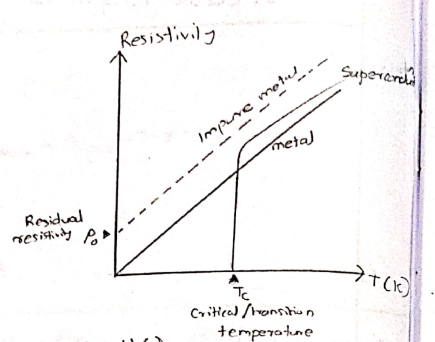
\includegraphics[max width=\textwidth]{rs}

	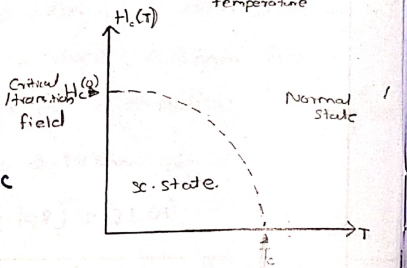
\includegraphics[max width=\textwidth]{ht}

	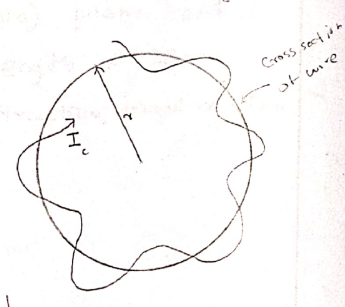
\includegraphics[max width=\textwidth]{wire}
\end{minipage}

\usubsection{Meissner effect}

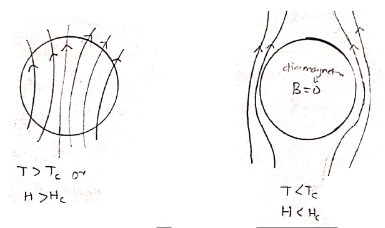
\includegraphics[max width=.8\linewidth]{meissner}

Meissner effect is the expulsion of a magnetic field from a superconductor during its transition to the superconducting state when it is cooled below the critical temperature

\usubsection{Classification of superconductors}

\begin{longtblr}{
		colspec = {XX},
		% rowhead = 1,
		hlines,
		vlines,
		rowsep=6pt,
		colsep=5pt
	}
	\SetCell{c}\Large\textbf{Type - I}                                                                            & \SetCell{c} \Large\textbf{Type -II}                                                                                                            \\
	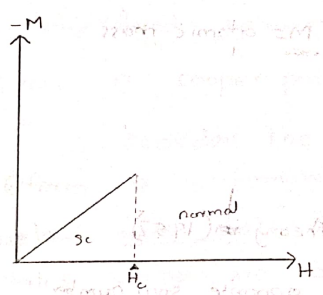
\includegraphics[max width=\linewidth]{type1}                                                                 & 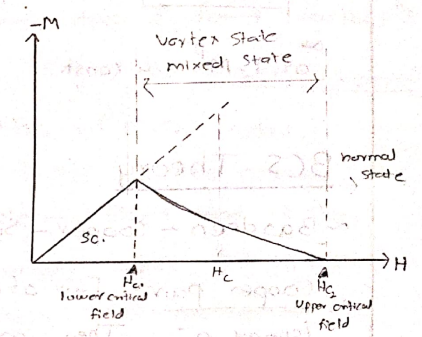
\includegraphics[max width=\linewidth]{type2}                                                                                                  \\
	Low transition temperature                                                                                    & High transition temperature                                                                                                                    \\
	Low \textit{Critical magnetic field} ($<1$ T)                                                                 & High \textit{Critical magnetic field} ($>1$ T)                                                                                                 \\
	Perfectly obey meissner effect                                                                                & Partially meissner effect                                                                                                                      \\
	They transition sharply and abruptly from a superconducting to a normal state under external magnetic fields. & Superconductivity gradually
	transition from a superconducting to normal state under external magnetic fields. At lower critical magnetic field ($H_{C1}$), it starts losing its superconductivity. At upper critical magnetic field ($H_{C2}$), it completely loses its superconductivity. \\
	Doesn't show \textit{flux pinning}                                                                            & Doesn't show \textit{flux pinning}                                                                                                             \\
	These are completely diamagnetic                                                                              & These are not completely diamagnetic                                                                                                           \\
	Exhibits single critical magnetic field                                                                       & Exhibits two critical magnetic field                                                                                                           \\
	Easily lose the superconducting state by low-intensity magnetic field.                                        & Does not easily lose the superconducting state by external magnetic field.                                                                     \\
	Also known as soft superconductors                                                                            & Also known as hard superconductors.                                                                                                            \\
	BCS theory can be used to explain the superconductivity of type-I                                             & BCS theory cannot be used to explain the superconductivity of type-II                                                                          \\
	Examples: Al, Hg, Pb, Zn,...                                                                                  & Examples: Zr, Nb, V, NbTi, Nb$_3$Sn, etc.                                                                                                      \\
\end{longtblr}

\qa{1}{Calculate critical current for a wire of lead Having a diameter 1 mm of at 4.2 K, T$_c$ for lead is 7.18K, $H_c(0)=6.5 \times 10^4 \unit{A/m}$}{
	$$
		\begin{aligned}
			H_c(4.2 K)     & =H_c(0) \left\{1-\left(\frac{T}{T_c}\right)^2\right\}                      \\
			\SwapAboveDisplaySkip                                                                       \\
			               & =6.5 \times 10^4 \times\left(1-\frac{4.2^2}{7.18^2}\right)                 \\
			               & =42758 \unit{T}                                                            \\
			\therefore I_c & =2 \pi r H_c=2 \times 3.141 \times \frac{1 \times 10^{-3}}{2} \times 42758 \\
			               & =135\unit{A}
		\end{aligned}
	$$
}

\qa{2}{Calculate $I_c$ that flows through a long thin superconducting wire of Aluminium of diameter 10$^{-3}$ m, (H$_c$(T)=7.9 $\times$ 10$^3$ T)}
{
	\eqnleft{
		I_c=2\pi rH_c(T) = 2\times 3.141 \times \frac{10^{-3}}{2} \times 7.9 \times 10^3=24.8 \mathrm{~A}
	}
}

\usubsection{Isotope effect}
$T_c \times M^\beta$ is constant. Where $T_c$ = critical temperature, M = atomic mass and $\beta$ = correction constant = $\frac{1}{2}$
\begin{flalign*}
	 & \boxed{T_c \propto M^{-\beta}} &  &
\end{flalign*}

\qa{1}{For Hg, T$_c$=4.185 K, and isotopic mass = 199.5. If the isotopic mass changes to 203.4, calculate its critical temperature.}
{
	\begin{flalign*}
		 & T_c(Hg) \propto \frac{1}{\sqrt{M_{Hg}}}         &  & \\
		 & T_c(Hg) = \lambda \frac{1}{\sqrt{M_{Hg}}}       &  & \\
		 & \text{ie}\ 4.185=\lambda \frac{1}{\sqrt{199.5}} &  & \\
		 & \lambda = 4.185 \sqrt{199.5}                    &  &
	\end{flalign*}
	\begin{flalign*}
		\therefore T_c \text{ of Hg with mass 203.4 } & =\lambda \frac{1}{\sqrt{203.4}}          &  & \\
		                                              & =4.185 \times \sqrt{\frac{199.5}{203.4}}      \\
		                                              & =4.145K
	\end{flalign*}
}

\usection{BCS Theory}
Bardeen-Cooper-Schriffer theory (1957)
\begin{framed}
	\textbf{Cooper pair}: When electrons enters a positive-lattice they get trapped in the lattice due to attractive and repulsive forces. And they may exchange energy in the form of phonons. and form cooper pair if they happened to have opposite spin numbers.
	\bigbreak
	\textbf{Super electrons}: Pair of electrons that are bound to each other.
\end{framed}

\textbf{BCS Theory}: This theory could explain many observed effects such as zero resistivity meissner effect, isotope effect, etc. It is based on advanced quantum theory.
\doparindent
Consider an electron posing through a lattice of positive ions, the electron is attracted by neighbouring positive ions, form a positive ion core. This greately reduces the effect charges of electron. Due to the attraction between electron and ion core, lattice gets deformed. If another electron passes by the side of the assembly of first electron and ion core, it gets attracted to wards the assembly. The second electron interacts with first electron through lattice deformations. This interaction is due to exchange of virtual phonons between two electrons. The momentum is transferred between electrons. These two electrons together forms a cooper pair the electrons are known as \textbf{cooper electrons or super electrons}.

Consider the distribution of electron in metals (see fermi-dirac formula). At $T=0 K$ all the energy states below fermi level are completely filled and all the states above are completely empty. When two electrons are added to the metal at absolute zero, since all the quantum states with energies $E<E_{\text {fermi }}$ are filled, they're forced to occupy states having energies $E>E_{\text {fermi }}$. they forced to occupy states having energies $E>E_{\text {fermi }}$. Cooper showed that if there's an attraction between two electrons, they are able to form a bound state so that their total energy will be less than $2 E_{\text {fermi }}$. These electrons are paired to form a single system. This system is called cooper pair and the electrons are called cooper electrons. Their motions are co-related. The binding is strongest when the electrons forming the pair have opposite momenta and opposite spins. So all the electron pairs lying in the neighbourhood of fermi surface form super electrons. These super electrons are responsible for superconductivity.
\begin{framed}
	\noparindent
	\textit{Fermi-dirac equation:}
	\begin{flalign*}
		\hspace{1cm} f(E)=\frac{1}{e^{\left(E-E_f\right) /\left(\sigma_E\right)}+1} &  &
	\end{flalign*}

	\textbf{Fermi surface}: Surface in reciprocate space which separates occupied a unpained electron
\end{framed}

\usection{Nanomaterials}
\ussubsection{Classification}
\begin{itemize}
	\item Based on dimension:
	      \begin{itemize}
		      \item ID-material or thin films (if any one of the dimension is $<10^{-9}$ m)
		      \item 2D-material or thin wires (if any two of the dimension are $<10^{-9}$ m)
		      \item 3D-material or quantum dots (if all dimensions are $<10^{-9}$ m)
	      \end{itemize}
	\item Based on structure:
	      \begin{itemize}
		      \item Fullerene
		            \begin{itemize}
			            \item Single walled carbon nanotubs
			            \item Double walled carbon nanotubs
		            \end{itemize}
		      \item Nanomaterials (general terms for inorgoric structures)
		            \begin{itemize}
			            \item Nanoparticle
			            \item Nanopowder
			            \item Nanocrystal
			            \item Nanoring
			            \item Nanoshell
		            \end{itemize}
	      \end{itemize}
\end{itemize}

\begin{framed}
	\noskipqa{
		Why nanomaterial show excellent/different properties?
	}
	{
		\begin{itemize}
			\item \textbf{Surface area to volume ratio}: When this increases, more atoms will be in surface and becomes highly energetic and reactive due to unsatisfied bonds
			\item \textbf{Quantum confinement effect}: Since electrons are confined to small volume, density increases a becomes night reactive.
		\end{itemize}
	}
\end{framed}
\usubsection{Fullerene}
\doparindent
Fullerene are a class of allotropes of carbon which are graphene sheets rolled into tubes or hollow spheres. Spherical fullerence are also called buck balls and cylindrical one called carbon nanotube or buckytubes. Fullerenes are similar in structure to graphite, but they may contain pentagonal rings. First fullerence discovered was Buckminster fullerene. $\left(C_{60}\right)$ in 1985.

Carbon nanoterbes are allotropes of Carbon with a Cylindrical nano structure. These are categorized as single walled nanotubes (SW) and multi walled (MW) nanotubes. These cylinchical carbon molecules a have nobel properties. They are potentially useful in many upplications in nanotechnology, electronics, optics and motorial Science. They exhibit extraordinary strength and unique electrical properties. They are efficient conductors of heat.

\usubsection{Nanoshell}
A nanoshell is a type of spherical nano particle consisting of a dielectric core which is covered by a thin metallic shell, which is usually a gold. Gold shelled nano particles with silica core are used in cancer therapy and bio. imaging enhancement.

\usubsection{Nanorodes}
These are one morphology of nanoscale objects. Their dimensions ranges from 1-100 nm. Standard aspect ratio (length/width). are 3-5. They can be produced by direct chemical synthesis. Applications of nanorodos include in-disply technology, mico-electro-mechanical systems, LED

\usubsection{Nanoring}
These are small ving formed crystals these are made up of fine nano belts. These that are rolled up as coils layer by layer with as many as 100 loops. The first handling was made of ZnO with thickness 10-30nm. with diameter of 1.4 microns. These have applications in MEMS and nano-electro-mechonial systers (NEMS).

\usection{Smart materials}
\usubsection{Liquid Crystal}
Liquid crystals is a state of matter frow have properties bowen "crystal and "liquid. It is sometimes difficult to determine whether a material is in a erystal is in liquid/liquid crystalline state Substance that are not is ordered as a solid yet have some degree of alignment are properly called liquid crystals

LC materials generally have several common characteristics. Rod like molecular structure, rigidness along long axis, and strong dipoles. Distinguishing characteristics of liquid crystelline state is the tendency of its molecules to point along a common axis called 'director'. ie, liquid crystal is a substance that flows like a liquid but maintains Some of the ordered structural characteristics of crystals.

Under certain circumstances LC have liquid like behaviour and during others, they have opposite behaviors. Most LC compounds exhibit polymorphism, a condition where more than one phase is observed in LC state.

The following parameters describe LC structure:
\begin{itemize}
	\item Positional order
	\item Orientational order
	\item Bond orientational order
\end{itemize}
\medskip
\begin{adjustwidth}{-10pt}{0pt}
	\begin{itemize}
		\item \term{Positional Order} refers to extend to which an average molecule or group of molecules show translational symmetry as crystalline materials shows.
		\item \term{Orientational Order} represents the tendency of the molecules to align along the director on a long range basis.
		\item \term{Bond orientational Order} describes a line joining the centers of nearest neighbouring molecules without requiring a regular spacing along that line.
	\end{itemize}
\end{adjustwidth}

% Metallic glasses, Shape memory alloys- optical, electrical magnetic and
% mechanical properties-applications.
\end{document}